NeXus is an effort by an international group of scientists to define a common data exchange and archival format for neutron, X-ray and muon experiments. NeXus is built on top of the scientific data format HDF5 and adds domain-specific rules for organizing data within HDF5 files.

\begin{figure}
\caption{A typical nexus file layout with shape definition}
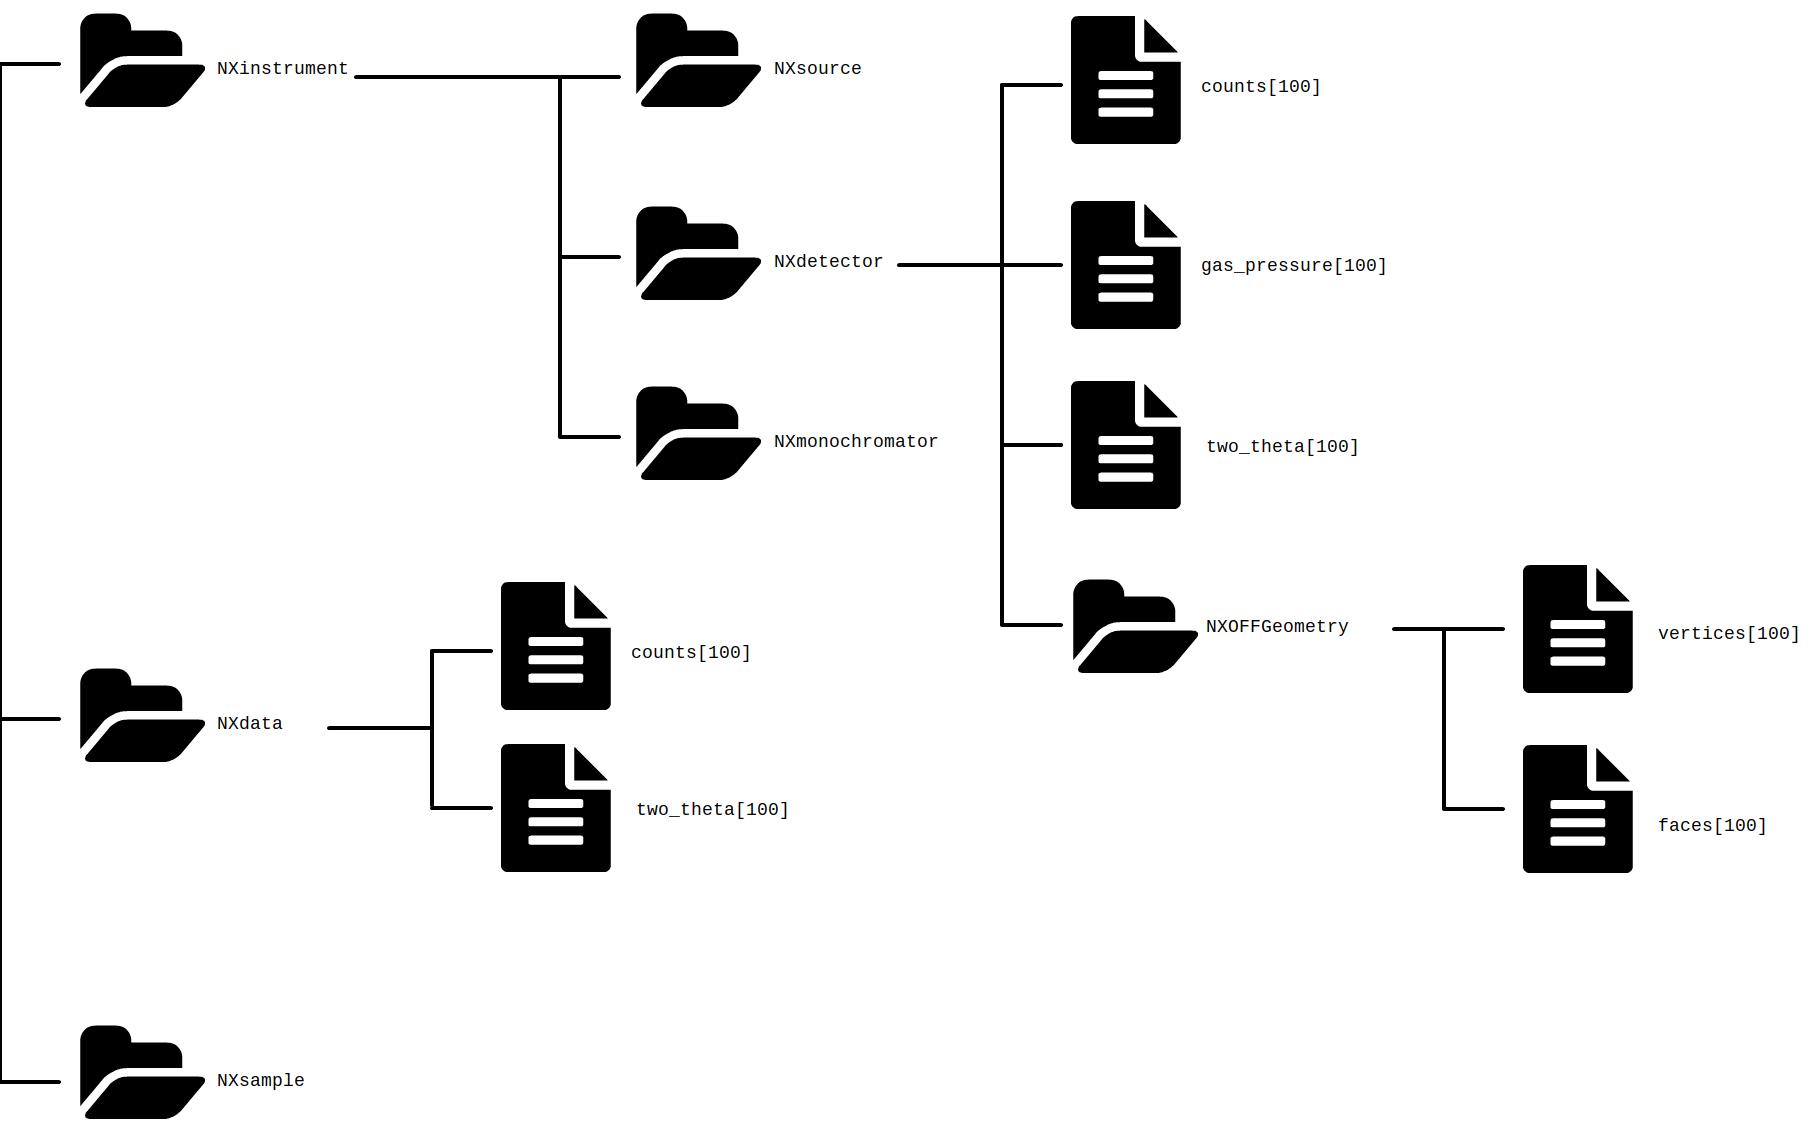
\includegraphics[width=\linewidth]{nexusdiagram.png}
\end{figure}

A recent addition to the NeXus standard means components that are used in experiments can specify shape definition to describe their placement, size and geometry. Transformations (NXtransformations) can be applied to these components when their position changes during or before the experiment. 

The NeXus file format arose out of a desire to describe the configurations of neutron and x-ray experiments in a way that is ``facility-neutral." An advantage is that this allows for greater openness in scientific research. However, the format is not particularly easy to understand for the unitiated and scientists would much rather get their data and get on with their day. The NeXus Constructor is the result of a collaboration between software developers based at ISIS and the ESS in order to make a tool that allows scientists to easily examine and modify the contents of NeXus files.
